\chapter{Background}

\section{Related Work}
A common approach to treating imperfect information games (IIG) is to create a rule based player, also known as a
heuristic player.
These players often do not perform very well, even when domain experts give their insight and are often used as
baselines for evaluation.
If they are however paired with Monte-Carlo-Tree-Search(MCTS) to find strategies they can reach par-human level as
shown by Bergh et al. in 2017 for the game of Hanabi\cite{hanabi} for the game of Hanabi.\\
Monte-Carlo(MC) methods however have been the gold standard for many years.
Ginsberg used traditional Monte-Carlo sampling to build an expert Bridge player back in 2001, which shows the power
of the method \cite{gib}.\\
However even basic MC-Simulation can produce decent results with little computing power as shown by Mizukami et al.
with the popular game of Majong \cite{mahjong}.
When MCTS is extended with \textit{Upper confidence bounds} as tree policy, which is the most common approach,
human-par play can be achieved Doppelkopf \cite{Doppelkopf}, similar in many regards to Schafkopf.\\
%[ISMCTS]
For more examples and a general overview see the review from Niklaus et al. \cite{niklaus2019survey}
\newline
In terms of reinforcement learning approaches there are the results from DeepMind's Alpha Star, a self-play learning
agent for the real time strategy computer game Starcraft.
They showed how imitation learning, a method of training an initial network with games of expert players, can even find
winning strategies in an action space of 10\textsuperscript{26}. \cite{Vinyals2019}\\
Imitation learning is certainly a viable strategy, but often the data is not readily available or the quality is
lacking.
\newline
The most relevant findings to this work is the agent of Charlesworth for the game Big2, a four player card game
.\cite{Charlesworth2018}
He trained an agent using self play and the recent Proximal Policy Algorithm by OpenAI \cite{Schulman2017} and
achieved human-par play.
Interestingly he achieved his results with a significant smaller batch size compared to Bansal et al.
\cite{Bansal2017}, which trained a variety of multi-agent environments in 3D, but whether this is due to
difference in environments or other factors is unclear.
It shows at least the robustness of Proximal Policy Optimisation.


\section{Neural Networks}
Machine learning consists of three approaches to problem-solving: Supervised learning, unsupervised learning and
reinforcement learning.
We will focus on the latter one, as reinforcement learning enables agents to learn complex behaviour through
exploration within a game environment.
In this chapter I will briefly explain the key concepts and methods of reinforcement learning that allow our model
learn the game of Schafkopf.
For this we will explain neural networks, their components and internal mechanisms, the reinforcement learning approach,
Proximal Policy Optimisation, which is the training algorithm used in our experiments, and Actor-Critic models.
\newline
A \textbf{Neural Network (NN)} is an attempt to imitate the complex behaviour of the human brain that
enables us as humans to learn complex skills.
The human brain consists of billions of neurons, the basic building block inside the nervous system, that are
interconnected to form large networks, capable of processing an input signal,for example a visual stimulus, into an
output.\\

\subsection{Artificial Neuron}
To imitate this we define an artificial neuron, with the goal of creating a type of switch to process an input signal
to an output, which could again be connected to further neuron.
To do so, we give the artificial neuron an input, a weight associated with that input,an activation function and an
output.
A neuron may have multiple inputs as well as outputs and the connection between the output of one neuron to the input
of another neuron is called an edge, which in turn may have their own weights.
The output signal is calculated by passing the sum of all weighted input signals through the activation function and
can be express by the following formula:
\newline
\begin{center}
    \begin{math}
        \boxed{
            \begin{aligned}
                &\textrm{Let } k\textrm{ be the neuron }k,&\\
                &\textrm{let } n \textrm{ be the number of inputs }x,&\\
                &\textrm{let } w \textrm{ be the weight,}&\\
                &\textrm{and let }\phi \textrm{ be the activation function}&\\
                &y\textsubscript{k} = \phi (\sum_{i=0}^n w\textsubscript{kn}x\textsubscript{n})
            \end{aligned}}
        \caption{Formula to calcualate neuron output }
        \label{neuronactivation}
    \end{math}
\end{center}
There are a number of possible activation functions that can be used, but for our purpose we will look at
\textbf{Rectified Linear Unit (RELU)} and the \textbf{Softmax}.\\
\newline
\textbf{ReLU} is a simple activation function that forwards the input, if its positive, otherwise zero.
The \textbf{ReLU} function is formulated using:

\begin{center}
    \begin{math}
        \boxed{
            \begin{aligned}
                &\textrm{Let } x \textrm{ be the input of a \textbf{ReLU}}\\
                &f(x) = max(0,x)
            \end{aligned}
        }
        \caption{Definition of \textbf{ReLU} activation function}
        \label{activationRelu}
    \end{math}
\end{center}
\textbf{ReLU}, when compared to the more tradition Sigmoid activation function, has proven to be favourable in terms
of computational efficiency and performance, when applied to deep neural networks. \cite{krizhevsky2012imagenet}
For this reason we exclusively use \textbf{ReLU} in all input and hidden layers.
\\
\textbf{Softmax} is a useful activation function for output layers, as they transform any input regardless of
absolute size to an output that is within [0,1].
The output of an output layer with \textbf{Softmax} is a normalised probability distribution, where each neuron in
the layer has a probability, and the sum of all probabilities is 1.
The definition of \textbf{Softmax} is the following:
\begin{center}
    \begin{math}
        \boxed{
            \begin{aligned}
                &\textrm{Let } z \textrm{ be the vector of } N \textrm{ inputs} \\
                &f(z)_{i} = \frac{e^{z_{i}}}{\sum_{j=1}^{N} e^{z_{j}} }
            \end{aligned}
        }
        \caption{Definition of the \textbf{Softmax} activation function}
        \label{activationSoftmax}
    \end{math}
\end{center}
\newline
Now that we defined a neuron, we can use multiple neurons to form a layer, which in turn can be connected in sequence
to form a \textbf{NN}.
The minimal architecture of a network consists of three layers, whereas the middle layers are named hidden layers:
\[\text{Input layer}\Rightarrow\text{Hidden layer}\Rightarrow\text{Output layer}\]
\newline
Between adjacent layers, every neuron's input is connected to the outputs of every neuron in the previous layer and
vice versa for the following layer.
See Fig. \ref{fig:architecture} for an example.
\newline

\begin{figure}[h!]
    \centering
    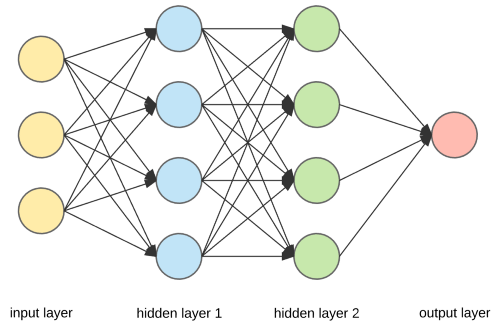
\includegraphics[scale=0.5,]{neuralnetlayer}
    \caption{Example architecture of a neural network with input,2 hidden and output layers}
    \label{fig:architecture}
\end{figure}
This kind of architecture is called \textbf{feed forward NN}, due to the process of passing an input linearly through
the network to the output, and will be used exclusively in our experiments.\\

\subsection{Policy}
The strategy for an agent to use inside an environment is called a \textbf{Policy}($\pi$).\\
The environment in our case is the game of Schafkopf, where an agent receives information about the current game
state(\textit{s}) at the time of his action that, which we use as input in our NN to make a decision on what action
(\textit{a}), in our case an action in the form of a valid card from our hand, to take.
At the end of each a hand we collect a reward(\textit{r}), which our policy over time tries to maximise.
\newline
An environment like ours can be described as \textbf{Markov Decision Process}, for which we define a four-tuple
consisting of a set states \textit{S}, a set of actions \textit{A}, a probability of our action \textit{a} as
\textit{P\textsubscript{a}} and a reward that results of that action \textit{R\textsubscript{a}}.\\
Set \textit{A} includes all the valid cards we can play in state \textit{s}.
Thus, we can define our policy as a function that takes a state and returns the probability of an action a value
function that predicts our reward \textit{r} for action \textit{a}:
\begin{center}
    \begin{math}
        \boxed{
            \begin{aligned}
                \pi(s)&\rightarrow P(a)\\
                f(s,a)&\rightarrow r_{a}\\
            \end{aligned}}
    \end{math}
\end{center}
Ideally we would want our policy to be optimal, for which we require a method of updating our NN using the
experiences and rewards we gained through interaction with the environment.
By optimal we understand, that from all states \textit{s\textsubscript{i}} we maximise the reward \textit{r}.
\newline
The process of updating a NN is called \textbf{Backpropagation}.\\
The idea is to adjust the weights of the networks neurons using a loss function, which calculates the error of our
predicted reward and our actual received reward.
Commonly used is the \textbf{Mean Square Error(MSE)}:
\begin{center}
    \begin{math}
        \boxed{
            MSE = \frac{1}{n} \sum_{i=1}^n(Y_{i}-\hat Y)^2
        }
    \end{math}
\end{center}
Ideally the \textbf{MSE} is zero, indicating that our predicted rewards are equal to the received rewards.
If not we use \textbf{Backpropagation}, which calculates the partial derivative of the total error and adjusts the
weights by traversing backwards through the NN.


\section{Actor-Critic}
The \textbf{Actor-critic} is a method of designing NNs that has a policy structure, known as the \textit{actor}
and a value structure, known as the \textit{critic}.
The \textit{actor} chooses an action for a given state, whilst the \textit{critic} evaluates the action taken.
\begin{figure}[!ht]
    \centering
    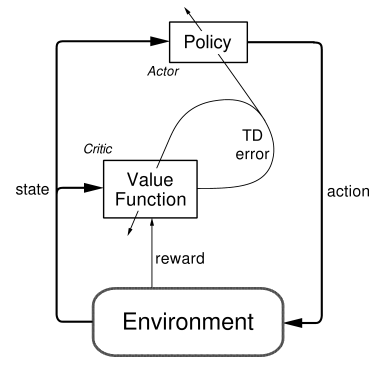
\includegraphics[scale=0.5]{actorcritic}
    \caption{Representation of an Actor-Critic model interacting with an enviroment \cite{actorcritic}}
\end{figure}


\section{Self-Play Learning}
\textbf{Self Play} learning describes the process of an agent that collects the training data itself by playing
himself, unlike in supervised learning, for which a labeled dataset needs to be provided.
The agent can figure out what works, and what does not, by stochastic exploration.
This way of generating experiences is what propelled Google's Alpha Zero to new heights and produced new strategies
modern chess engines and humans alike did not know about.\cite{Silver2017}


\section{Proximal Policy Optimisation}
\textbf{Proximal Policy Optimisation(PPO)} is a state of the art policy learning algorithm by OpenAI
.\cite{schulman2017proximal}\\
With previous algorithms it was sometimes hard to get good results due to the fact, that there were a lot of
moving parts in terms of parameter tuning of stepsizes.
If the stepsize is too low no progress is made, and vice versa one runs the risk of drowning the model in noise or
large policy updates result in a loss of progress.
Additionally, this problem is compounded by the need of tuning two cost functions for both \textit{actor} and
\textit{critic}.
\textit{PPO} solves this by introducing a trust region, that dynamically hinders the policy to make to large of a
step in either direction.
\begin{figure}[!ht]
    \centering
    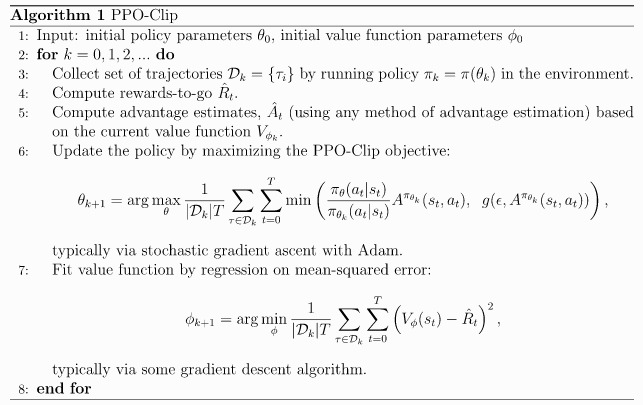
\includegraphics[scale = 0.5]{ppopseude}
    \caption{PPO-Pseudocode \cite{actorcritic}}
    \label{Pseudocode}
\end{figure}
\\
In Fig. \ref{Pseudocode} we can see in step 6 the function \textit{g}, also called the clipping function.
\begin{center}
    \begin{math}
        \boxed{
            g(\varepsilon,A) = \left\{\begin{matrix}
            (1+\varepsilon)
                                          & A \geq 0 \\
                                          (1-\varepsilon) & A < 0
            \end{matrix}\right.
        }
    \end{math}
\end{center}
If the advantage of an state-action pair is positive our policy will favour this action in the future, however only
to the extend of $\epsilon.$\\
Similary, if the advantage is negative, an action will fall out of favour in the future, but by how much is agian
limitied by $\epsilon$.
This stops our policy of making to big of change in one update step, and helps deal with noise, of which there is a
lot in stochastic games, since good decisions will not lead to good outcomes everytime.